\begin{problem}[11]
分析定常管流问题中的摩擦系数; 什么情况下可不考虑密度的影响? 说明其物理原因.
\end{problem}
% --------------------------------------------------------------------
\begin{solution}
\begin{minipage}[c]{0.8\linewidth}
摩擦系数$c_d$可以用单位面积摩擦力与动压之比定义. 因此摩擦系数$c_d$与管径$d$, 流体密度$\rho$, 平均流速$v$, 粘性系数$\mu$有关:
\[
c_d = f(d,\rho, v, \mu)
\]
\end{minipage}
\begin{minipage}[c]{0.2\linewidth}
\begin{center}
\usetikzlibrary{calc,intersections,through,backgrounds}
\usetikzlibrary{decorations.pathreplacing,decorations.pathmorphing,arrows}
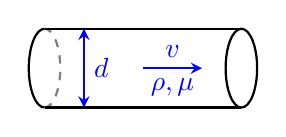
\begin{tikzpicture}
	\draw[dashed,color=gray, thick] (0,0) arc (-90:90:0.2 and 0.5);% right half of the left ellipse
	\draw[thick] (0,0) -- (2.5,0);% bottom line
	\draw[thick] (0,1) -- (2.5,1);% top line
	\draw[thick] (0,0) arc (270:90:0.2 and 0.5);% left half of the left ellipse
	\draw[thick] (2.5,0.5) ellipse (0.2 and 0.5);% right ellipse
    \draw[<->, >=stealth, thick,blue](0.5,0)--(0.5,1) node[right,midway] {$d$};
    \draw[->, >=stealth, thick,blue](1.25,0.5)--(2,0.5) node[above,midway] {$v$} node[below, midway]{$\rho, \mu$};
\end{tikzpicture}
\end{center}
\end{minipage}
上式中各物理量的量纲分别为: $c_d$为无量纲量, $[d]=L$, $[\rho]=ML^{-3}$, $[v]=LT^{-1}$, $[\mu]=ML^{-1}T^{-1}$. 取$\rho$, $v$, $d$为基本量, 且作为本问题的单位系统, 用以度量问题中的各量, 于是上式转化为
\[
c_d = f\bigg(1,1,1,\frac{\mu}{\rho v d}\bigg) = f\bigg(\frac{\rho v d}{\mu}\bigg)=f(\mathrm{Re})
=f\bigg(\frac{\rho}{\mu/(vd)}\bigg)\]
显然当雷诺数$\mathrm{Re}=\frac{\rho}{\mu/(vd)}$较小时, 可不考虑密度. 雷诺数$\mathrm{Re}$较小时, 流动为层流, 流体中的每个质点都做匀速运动, 相对于粘性力, 流体受惯性力影响较小, 因此这种情况下可以不考虑惯性即密度的影响.
\end{solution}
